\documentclass[a4paper]{article} 
\usepackage{graphicx,amssymb} 
\usepackage{amsmath,bm,bbm}
\usepackage{hyperref}
\usepackage{cite}
\usepackage[left=35mm, right=35mm, top=15mm, bottom=20mm, noheadfoot]{geometry}

\textwidth=15cm \hoffset=-1.2cm 
\textheight=25cm \voffset=2cm 

\pagestyle{empty} 

\date{} 

\def\keywords#1{{\bf Keywords: }{#1}}

\begin{document}
\thispagestyle{empty}

\title{\textbf{Information Theory and Computational Statistics in Signal Processing and Analysis --- Optimized Implementations in \texttt{R}}}

\author{Eduarda T. C. Chagas, Alejandro C. Frery \\ 
	Universidade Federal de Alagoas \\ \\ 
	\tt{etcc@ic.ufal.br}
}

\date{}
\maketitle\thispagestyle{empty} 


\begin{abstract}
A time series is a set of data obtained sequentially through observations over a period of time, not precisely partitioned in equal spaces of time, resulting from the operation of a system.
Such system may be comprised of any mixture of deterministic and stochastic components. 
It is of paramount importance to detect and characterize structural dependence patterns in such data sets.

Being a solid area in Statistics, the analysis of time series has a applications in the most diversified areas, such as bank data analysis, vehicular network characterization, seismic data, among many others.

There are several ways to perform the analysis of these data, however the vast majority of them are composed of language libraries dedicated to the development of mathematical calculations, which require a minimum knowledge of them.
In this way, the project aims to provide a friendly graphical tool with efficient, fast and good numerical quality functionalities that allows for interactive and exploratory analysis of the data through techniques derived from Information Theory.
The fundamental requirements are portability with respect to operating systems and hardware architectures, and the use of FLOSS (Free / Open Source Software) tools.

%In carrying out the process of time series analysis, we have as main objective to determine patterns in the midst of inherent randomness so characteristic, so that it becomes possible the analysis and consequent decision making based on these results.
%Based on the Information Theory, specific properties of a
%temporal series, contributing to their better study.

Time series $\bm x = (x_1, x_2, \dots, x_n)$ are transformed in sequences of symbols by the technique of Bandt \& Pompe approach~\cite{PermutationEntropyBandtPompe}.
Each symbol is a nonparametric mapping between groups of $N$ values and ordinal patterns.
We then analyze frequency distribution of the possible $N!$ symbols. 

We then extract quantifiers, such as entropy, stochastic distances to an equilibrium distribution, and the statistical complexity from the histogram.
In particular, the Shannon entropy is the metric used to measure the system disorder that gave rise to the $\bm x$ data; it is computed them from $\bm h = (h_1, \dots, h_{N!})$, the histogram of the proportions, as

\begin{equation}
H(\bm h) = -\sum_{i=1}^{N!} h_i\log h_i) ,
\label{eq:Entropia}
\end{equation}

where, by convention, $-\infty 0=0$.

A common reference distribution is the uniform over the $N!$ symbols: $\bm u=(1/N!,\dots,1/N!)$.
The Jensen-Shannon distance measures how close or far the underlying dynamics lie with respect to a process without information:

\begin{equation}
D(\bm h,\bm u) = \sum_{i=1}^{N!} \Big(h_i \log\frac{h_i}{u_i} +
u_i \log\frac{u_i}{p_i}
\Big),
\end{equation}
where $u_i=1/N!$.

We also calculate the statistical complexity, which seeks to find structures of interaction and dependence between the elements of the series:

\begin{equation}
C(\bm h, \bm u) = H(\bm h) D(\bm h, \bm u).
\end{equation}

Each time series can be thus represented by a point $(H(\bm h), C(\bm h, \bm u))$ in a compact subset of $\mathbbm R^2$: the Entropy-Complexity plane.
By means of such a tool it is possible to discover the nature of the series, determining if this is a chaotic, stochastic or deterministic sequence~\cite{Rosso2007}.

Although only the Shannon entropy and the Jensen-Shannon divergence were cited, the project provides other measures of entropy~\cite{salicruetal1993} and stochastic distances~\cite{StatisticalInferenceBasedonDivergenceMeasures}.

Our system promotes the analysis of the underlying dynamics of time series.
It enriches such analysis by a number of descriptors, aiding a variety of applications of the Bandt \& Pompe symbolization approach, for example, in the recognition of patterns of behavior in vehicular networks~\cite{CharacterizationVehicleBehaviorInformationTheory} and in the discrimination between stochastic and chaotic phenomena~\cite{DistinguishingNoiseFromChaos}.

\begin{figure}[hbt]
	\centering
	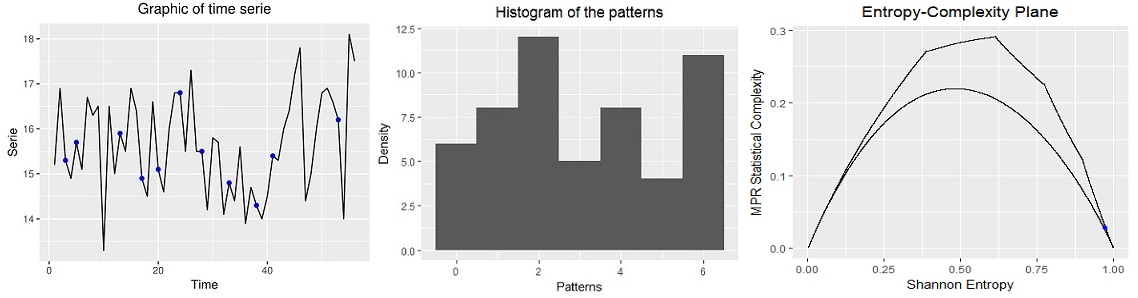
\includegraphics[width=1\columnwidth]{rplot}        
     \caption{Graphical representation of the analysis of a time series of annual production of barley per acre.}
\end{figure}

\end{abstract}

\keywords{Time series, information theory, \texttt R language.}

\bibliographystyle{unsrt}
\bibliography{ref}

\end{document}